\documentclass[tikz,border=3pt]{standalone}
\usepackage{tikz}
\usetikzlibrary{positioning,arrows.meta}

\begin{document}
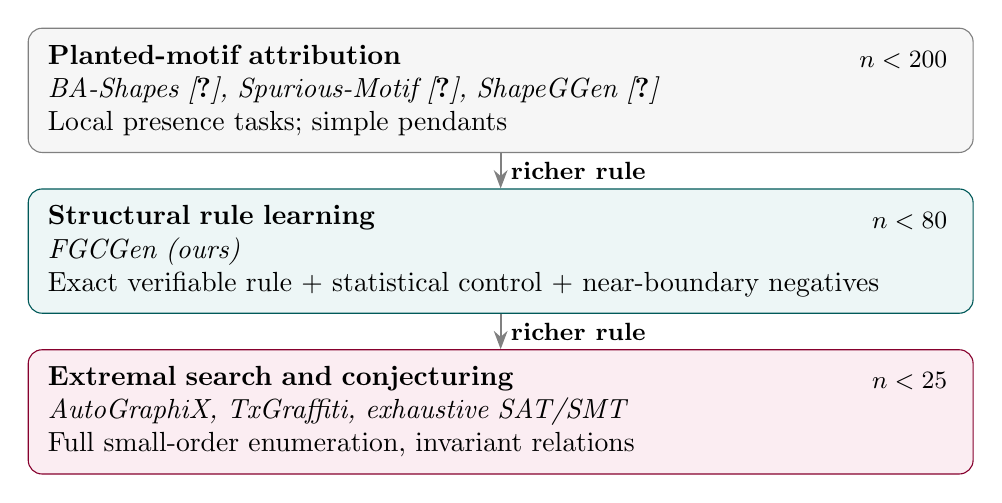
\begin{tikzpicture}
[
box/.style={draw, rounded corners=5pt,
	minimum width=12cm, text width=11.5cm,
	inner sep=6pt, align=left},
>=Stealth
]

\node[box, fill=gray!7, draw=gray] (a) {
	\textbf{Planted-motif attribution}\\
	\textit{BA-Shapes \cite{TODO}, Spurious-Motif \cite{TODO}, ShapeGGen \cite{TODO}}\\
	Local presence tasks; simple pendants
};

\node[box, fill=teal!7, draw=teal!70!black,
below=0.45cm of a] (b) {
	\textbf{Structural rule learning}\\
	\textit{FGCGen (ours)}\\
	Exact verifiable rule + statistical control + near-boundary negatives
};

\node[box, fill=purple!7, draw=purple!70!black,
below=0.45cm of b] (c) {
	\textbf{Extremal search and conjecturing}\\
	\textit{AutoGraphiX, TxGraffiti, exhaustive SAT/SMT}\\
	Full small-order enumeration, invariant relations
};

\draw[->, gray, thick] (a) -- node[right, black, font=\bfseries\small]
{richer rule} (b);

\draw[->, gray, thick] (b) -- node[right, black, font=\bfseries\small]
{richer rule} (c);

\node[anchor=north east, font=\small\bfseries]
at ([xshift=-6pt,yshift=-5pt]a.north east) {$n<200$};

\node[anchor=north east, font=\small\bfseries]
at ([xshift=-6pt,yshift=-5pt]b.north east) {$n<80$};

\node[anchor=north east, font=\small\bfseries]
at ([xshift=-6pt,yshift=-5pt]c.north east) {$n<25$};

\end{tikzpicture}
\end{document}